\documentclass[conference]{IEEEtran}

\IEEEoverridecommandlockouts

\usepackage{cite}
\usepackage{amsmath,amssymb,amsfonts}
\usepackage{algorithmic}
\usepackage{graphicx}
\usepackage{textcomp}
\usepackage{xcolor}

\def\BibTeX{{\rm B\kern-.05em{\sc i\kern-.025em b}\kern-.08em
    T\kern-.1667em\lower.7ex\hbox{E}\kern-.125emX}}

\begin{document}

\title{Sequence Alignment and Parallel Programming}

\author{\IEEEauthorblockN{1\textsuperscript{st} Daniel Vail}
\and
\IEEEauthorblockN{2\textsuperscript{nd} Austin Traub}
\and
\IEEEauthorblockN{3\textsuperscript{rd} Tony Pham}
}

\maketitle

\begin{abstract}
In our project, we explore the parallelization of the algorithms used in sequence alignment based on dynamic programming. We researched the Needleman-Wunsch, the Smith-Waterman, and Hirschberg's algorithms. We then performed experiments attempting to parallelize them using the anti-diagonal technique and recorded our results. Our focus was on the Needleman-Wunsch algorithm since the Smith-Waterman algorithm is just a variation of it and Hirschberg's algorithm is a more space efficient version of it. In the end, we found that, when it comes to sequence alignment, the cost of parallelizing outweighs the benefits. This is due to the limitations of the anti-diagonal parallelization technique. The matrices used in the algorithm can only be filled in one anti-diagonal at time, and it has to be done in order. As a result, parallelization can only be done within each anti-diagonal.
\end{abstract}

\section{Introduction}
The purpose of this project is to explore the algorithms and related parallel programming techniques used in sequence alignment. Sequence alignment is a process in bioinformatics whereby DNA, RNA, or protein is aligned in way that produces an optimal match between the residues of the molecules being aligned. DNA and RNA are made of nucleotides, and proteins are made of amino acids. Nucleotides and amino acids are represented as letters, and it is the sequences of those letters that are being aligned.

Sequence alignment is typically used to study the functions of biological sequences. Similarity between two biological sequences usually indicate that those sequences perform the same function. Thereby, sequence alignment is a highly useful process when it comes to studying this.

There are two main types of sequence alignments: pairwise alignment and multiple sequence alignment \cite{chaudhary_liu_matta_yang_2005}. In a pairwise alignment, two sequences are compared and aligned. In a multiple sequence alignment, multiple sequences are aligned. This project will focus on algorithms for pairwise alignment. The typical application of pairwise alignment is to allow users to search a database for sequences similar to a specified input sequence. The input sequence is compared pairwise to each sequence in the database and the best matches are returned.

Alignments can be categorized further as either global or local. A global alignment is one that finds the best alignment for the entire sequence from beginning to end \cite{global_alignment}. This is useful for comparing closely related sequences. A local alignment is one that finds similarities in only local regions of the sequences \cite{global_alignment}. This is useful for when maybe only certain regions of the sequences being compared are similar. The project will look at algorithms for both global and local alignments.

What makes the sequence alignment problem difficult is the size of the sequences usually being compared. The typical size of a DNA sequence string in FASTA format, for example, can range from 40KB to 60KB \cite{naveed_siddiqui_ahmed}. Using a sequence alignment algorithm such as the Needleman-Wunsch Algorithm, which runs in O(MN), can take some time. In addition, doing this many times over while searching a database makes this process impractical. That is why it is important to look into ways in which sequence alignment could be parallelized.

The following is an example sequence alignment for the sequences TCGATA and AGATC:\\

\hspace*{1em}TCGATA\\
\hspace*{2em}–AGATC\\
 
The dash before the letter A in the second sequence in the alignment represents a gap. Gaps are indicative of insertions or deletions. Sequences may have been the same at some point in time and ended up diverging through mutations involving substitutions, insertions, or deletions \cite{settles_2008}. For example, the second sequence above could have undergone a mutation where T (the first letter) was deleted and C (the second letter) was substituted with an A.

Another possible alignment for the sequences above is as follows:\\

\hspace*{1em}TCGATA\\
\hspace*{2em}A–GATC\\

This example indicates that, in the second sequence, a mutation could have caused T (the first letter) to be substituted with A and C (the second letter) to be deleted. To determine which alignment is best, algorithms use a scoring system to assign a score to each possible alignment. Usually, the alignment with the highest score is the optimal alignment.

The existing algorithms for sequence alignment fall into three categories: dynamic programming based, heuristic-based, or a mixture of the two \cite{chaudhary_liu_matta_yang_2005}. The dynamic programming based algorithms breaks the problem into subproblems and finds a solution using the bottom up approach. In order words, the optimal alignments for the subsequences are found, and those are used to find optimal alignment for the overall sequences. The dynamic programming based solutions are computationally demanding, making them impractical when dealing with a great number of sequences \cite{chaudhary_liu_matta_yang_2005}. As a result, heuristic approaches are typically used to approximate the optimal alignment. These heuristic solutions typically use dynamic programming for only a portion of the sequence while using approximations to make the search space more manageable. The result is a faster and more efficient algorithm.

The focus of the project is to only explore existing sequential and concurrent algorithms for sequence alignment based on dynamic programming.

\section{Goals}
As stated before, the goal of this project is the explore existing sequential and concurrent algorithms for sequence alignment based on dynamic programming. We will attempt to implement these algorithms and explore the parallelization of them through experimentation.

\section{Existing Algorithms}
The following section presents some dynamic programming based algorithms for sequence alignment. The Needleman-Wunsch algorithm is used to find global alignments. The Smith-Waterman algorithm is used to find local alignments. And the Hirschberg algorithm is a space efficient modification of the Needleman-Wunsch algorithm.

\subsection{Needleman-Wunsch}
The Needleman-Wunsch algorithm uses dynamic programming to find the optimal global alignment between two sequences \cite{vladimir}. It finds the optimal alignment across the entire sequence. The algorithm is based on the idea that the overall optimal alignment of two sequences can be determined through determining the optimal alignments of their subsequences and building up from there. All possible alignments of the two sequences are determined, and a score is given to each to rank it. The alignment with the highest score is the most optimal one.

The algorithm involves the use of two matrices: the score matrix and the traceback matrix. It can be broken down into three main parts: the initialization of the two matrices, the calculating of the scores and directions in the two matrices, and using the traceback matrix to determine the optimal alignment.

The score matrix is used to store the score for each alignment. The traceback matrix is used to store the direction from which each score came from. Each score in the score matrix is calculated based on a previously calculated neighboring score. The directions in the traceback matrix are used to trace and determine the highest scoring alignment. Fig.~\ref{1} is an example score matrix, and Fig.~\ref{2} is its corresponding traceback matrix.

\begin{figure}[htbp]
\centerline{\scalebox{.75}{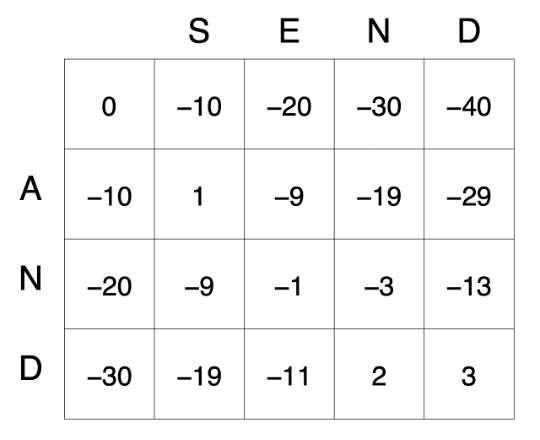
\includegraphics{Figures/1.png}}}
\caption{Example score matrix. \cite{vladimir}}
\label{1}
\end{figure}

\begin{figure}[htbp]
\centerline{\scalebox{.72}{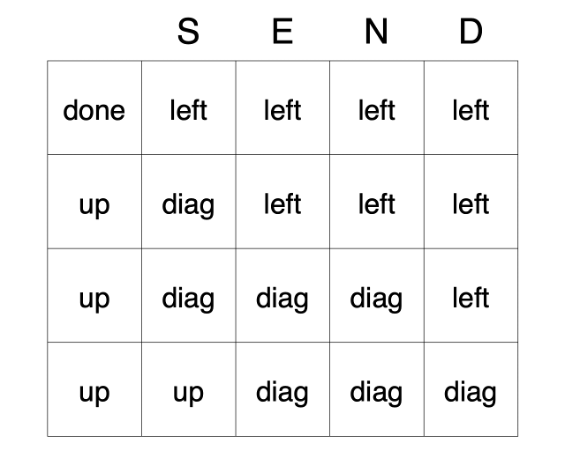
\includegraphics{Figures/2.png}}}
\caption{Example traceback matrix. \cite{vladimir}}
\label{2}
\end{figure}

A scoring scheme needs to be picked to help calculate the scores. A basic example scheme is to use +1 for a match, -1 for a mismatch, and 0 for a gap. A match occurs when two letters match. A mismatch is when the letters do not match. And a gap is where the letter from one sequence is lined up with a gap, corresponding to an insertion/deletion. Inserting a gap into a sequence shifts it, causing a letter from the other sequence to match with the gap.

A substitution matrix can also be used to define the scoring scheme more thoroughly. Using a substitution matrix, different matches/mismatches could be assigned different substitution scores. For example, a C-C match could be assigned a +1 while a T-T match could be assigned a +2. Below in Fig.~\ref{3} is an example substitution matrix. Here, all the matches are assigned +1 while all the mismatches are assigned -1. For example, the value 1 in row 2 column 2 indicates that a C-C match should have a substitution score of 1.

\begin{figure}[htbp]
\centerline{\scalebox{.72}{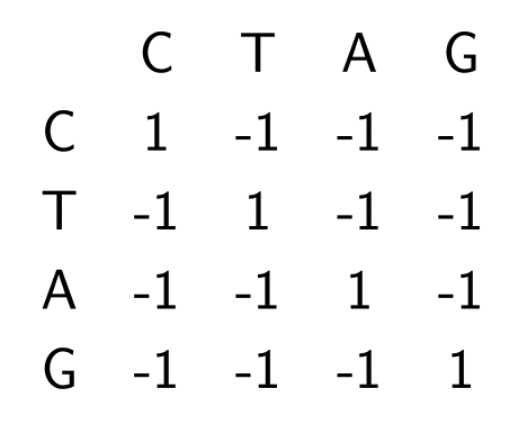
\includegraphics{Figures/3.png}}}
\caption{Example substitution matrix. \cite{vladimir}}
\label{3}
\end{figure}

To determine the score for a cell in the score matrix, the scores of the neighboring cells to the left, above, or on the top left of the current cell are taken into account. The subscore of the current cell, determined by the scoring scheme, is added to the score of each of those neighboring cells individually. The highest result out of the three is chosen as the score for the current cell. Going to the cell on the left means adding a gap to the letter on the sequence placed on the left side of the matrix. The gap penalty should be added here. Going to the cell above means adding a gap to the letter on the sequence at the top of the matrix. The gap penalty should be added here in this case. Going diagonally to the top left means that a gap was not added. Here, the match score should be added for a match, and the mismatch score should be added for a mismatch. The scoring system is represented by the recursive relation in Fig.~\ref{4}, where \textit{s(i, j)} is the substitution score and \textit{g} is the gap penalty. Fig.~\ref{5} demonstrates this relation visually on a score matrix.

\begin{figure}[htbp]
\centerline{\scalebox{.72}{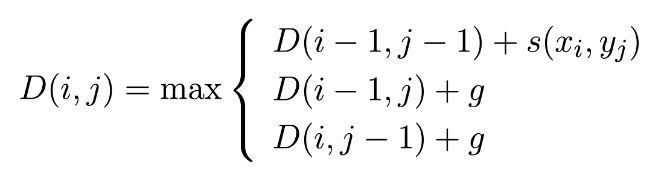
\includegraphics{Figures/4.png}}}
\caption{Recursive relation to determine the score. \cite{vladimir}}
\label{4}
\end{figure}

\begin{figure}[htbp]
\centerline{\scalebox{.72}{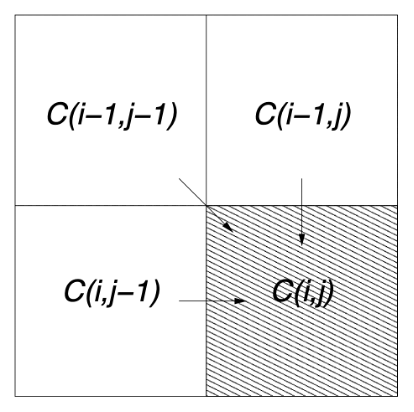
\includegraphics{Figures/5.png}}}
\caption{Determining the score on the matrix. \cite{vladimir}}
\label{5}
\end{figure}

The directions in the traceback matrix are either Left, Up, or Diagonal (for top left). The direction for each cell depends on which of the three neighboring cells was used to determine the final score for it. For example, if the final and highest score for a cell in a score matrix was calculated using the cell above it, the corresponding cell in the traceback matrix would have the value U for Up.

To demonstrate, in the score matrix below in Fig.~\ref{6}, the score for row 2 column 2 (A-A) is determined to be 2. This matrix uses -2 for the gap penalty, -3 for a mismatch, and 2 for a match. Starting at row 2 column 2, going left to row 2 column 1 means adding a gap to the sequence on the left side of the matrix. The gap penalty is -2, so the total score for going left is the sum of the left cell and the gap penalty. That is, -2 + -2 = -4. Similarly, going up to row 1 column 2 means adding a gap to the sequence at the top of the matrix. The total score here is also -2 + -2 = -4. Lastly, going diagonally to row 1 column 1 means not adding a gap. The current cell is a match since it represents the pair A-A; both the letters corresponding to the row and column of the cell are A’s. The score for a match is 2. Accordingly, the total score here is 0 + 2 = 2. Out of the three scores calculated, 2 is the highest, so it is chosen as the final score for the cell. Since the max score is calculated using the top left diagonal neighboring cell’s score, we set the corresponding cell’s value in the traceback matrix to D for diagonal. That is, we set the value of row 2 column 2 of the traceback matrix to D.

\begin{figure}[htbp]
\centerline{\scalebox{.72}{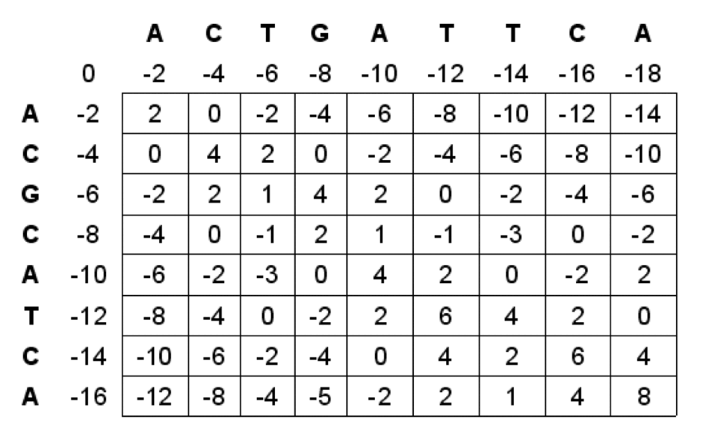
\includegraphics{Figures/6.png}}}
\caption{Another example score matrix. \cite{musso}}
\label{6}
\end{figure}

The scoring matrix is initialized by setting the top uppermost leftmost cell to 0. The gap penalty is then added incrementally both along the first row and first column. For example, in Fig.~\ref{6}, where the gap penalty is -2, the scores along the first row are 0, -2, -4, -6, -8, and so on. The scores along the first column are the same. These scores indicate the overall score for appending gaps to the beginning of each sequence. For instance, adding two gaps to the beginning of the left sequence above produces -{}-ACGCATCA. The corresponding score for this alignment is -4 since row 3 column 1 is -4.

Once all of the scores in the score matrix and the directions in the traceback matrix have been determined, the traceback matrix is used to produce the most optimal alignment between the two sequences. The traceback begins at the bottommost rightmost cell. The trace then moves either left, up, or diagonally from that point on. Movement is based on the direction stored in the traceback matrix. Moving left means adding a gap to the sequence on the left of the matrix. Moving up means adding a gap to the sequence at the top of the matrix. And moving diagonally means that the two letters for that cell are aligned and no gap is to be added. The traceback ends when the topmost leftmost cell is reached. Fig.~\ref{7} shows an example traceback matrix and its final path. The corresponding optimal alignment for the sequences SEND and AND is as follows:\\
 
\hspace*{1em}SEND\\
\hspace*{2em}A–ND

\begin{figure}[htbp]
\centerline{\scalebox{.7}{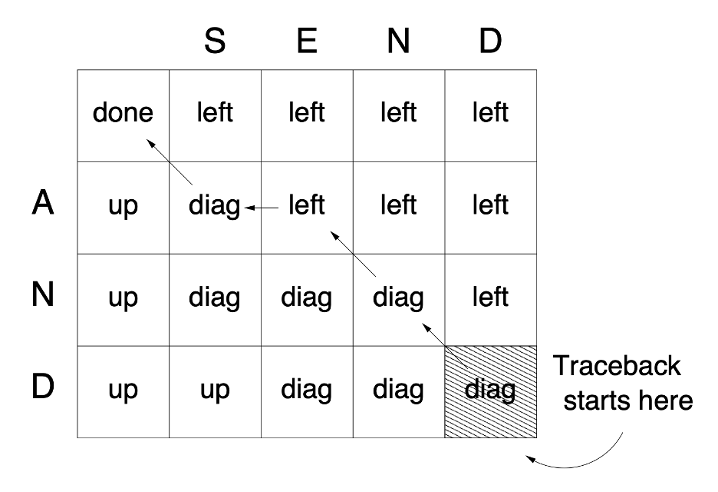
\includegraphics{Figures/7.png}}}
\caption{Another example traceback matrix. \cite{vladimir}}
\label{7}
\end{figure}

\subsection{Parallel Version of Needleman-Wunsch}
Naveed, Siddiqui, and Ahmed describes a method for parallelizing the Needleman-Wunsch algorithm \cite{naveed_siddiqui_ahmed}. This method involves two parts: the parallel initialization of the matrices used in the algorithm and the parallel calculation of the scores and directions that fill the matrices.

The score and traceback matrices each can be initialized by two separate threads. One thread can set the initial row column values (-1, -2, -3, … or Left) while the other thread can set the initial first column values (-1, -2, -3, … or Up). If the sequences are stored in the matrices as headers, they also can be stored in a similar parallel manner. One thread sets the first sequence across the top and the other sets the second sequence along the side.

As for the calculating the scores, the scores can be calculated anti-diagonally. This way, the calculations can be parallelized within each anti-diagonal. The scores in the first anti-diagonal are calculated first, then the second, the third, and so on. Fig.~\ref{8} below shows the anti-diagonals used in this technique. Calculating the scores in an anti-diagonal order is possible since each score is determined based on the cells left, above, or top left of it. The scores for the left, top, and top left cells for each cell will be already determined by the time we attempt to fill in the next anti-diagonal.

In Fig.~\ref{8} below, row 2 column 2 would be calculated first. Then row 2 column 3 and row 3 column 2 would be calculated next in parallel. Here, one thread can be used to calculate row 2 column 3 and another can be used to calculate row 3 column 2. The next calculations are row 2 column 4, row 3 column 3, and row 4 column 2 together in parallel. This pattern continues until the matrix is completely filled in.

\begin{figure}[htbp]
\centerline{\scalebox{.68}{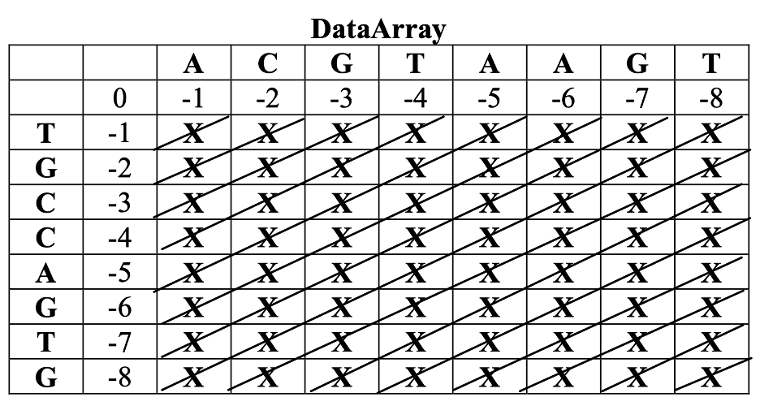
\includegraphics{Figures/8.png}}}
\caption{Sections that can be calculated in parallel. \cite{naveed_siddiqui_ahmed}}
\label{8}
\end{figure}

The limitation of this method is that the parallelization can be done only within each anti-diagonal. To start filling in the next anti-diagonal, the preceding anti-diagonal must already be all completed. Otherwise, there would not be enough information to calculate all of the scores for that anti-diagonal. The scores in each anti-diagonal is dependent on the scores in the preceding anti-diagonal.

According to the authors, the parallel version of the Needleman-Wunsch algorithm has a runtime of O(N+M) \cite{naveed_siddiqui_ahmed}. This is an improvement over the O(MN) runtime of the original algorithm.

\subsection{Smith-Waterman}
The Smith-Waterman algorithm is used to find the optimal local alignment between two sequences. It finds the optimal alignment based on local regions instead of the entire sequence. It is a variation of the Needleman-Wunsch algorithm. It differs from the Needleman-Wunsch algorithm in three ways. First, the first row and column of the score matrix is initialized with zeros. In the Needleman-Wunsch algorithm, initialization is based on the gap penalty. Second, if the final score for a cell is negative, it gets replaced with a zero. In the Needleman-Wunsch algorithm, negative scores are kept. And lastly, the traceback step starts at the highest score and stops when a zero is reached. In the Needleman-Wunsch algorithm, traceback starts at the last cell and ends at the first cell. Because the Smith-Waterman algorithm is a variation of the Needleman-Wunsch algorithm, it can be parallelized in the same way. That is, it can be parallelized by traversing anti-diagonally and calculating the scores in each anti-diagonal concurrently.

\subsection{Hirschberg}
Created in the mid-1970’s by Dan Hirschberg, Hirschberg’s algorithm is an improvement to the Needleman-Wunsch algorithm created at the beginning of that decade \cite{hirschberg_1975}. The goal of the algorithm is to find the optimal global sequence alignment of two strings. Hirschberg’s improvement on the Needleman-Wunsch algorithm comes from it being more spatially efficient. As stated in the above section, the runtime efficiency of Needleman-Wunsch is O(nm), where n and m are the lengths of the two strings respectively. Hirschberg’s algorithm has the same runtime. The difference is that Needleman-Wunsch uses O(nm) space, since it creates an n by m matrix, where n and m are the lengths of the sequences, whereas Hirschberg’s algorithm only takes O(min\{n,m\}) space by using binary recursion \cite{edit_distance_revisited}.

\section{Experiments}

This section describes in detail our attempts to parallelize the algorithms described above. All of our experiments were coded using Java. Our experiments for the Needleman-Wunsch algorithm also applies to the Smith-Waterman algorithm since the latter is a slight variation of the former.

\setcounter{subsection}{0}

\subsection{Needleman-Wunsch}
Naveed, Siddiqui, and Ahmed described a method to parallelize the Needleman-Wunsch algorithm in their paper but did not show an actual implementation \cite{naveed_siddiqui_ahmed}. We attempted to implement parallelized versions of the Needleman-Wunsch algorithm based on the anti-diagonal method described in their paper. The results of our experiments are described in this section.

For each of our experiments, we implemented and ran a sequential version of the algorithm alongside the parallelized version to compare the runtimes between the two. The sequential version that we implemented is the dynamic programming based algorithm described in the prior section. The main part of our sequential implementation is the fillMatrices() method, which fills up both the score matrix and traceback matrix for the two input sequences. After the initialization of the first row and first column of each matrix in the constructor, the matrices are filled from left to right starting from the top left based on the scoring system described in the prior section.

Fig.~\ref{9} shows the code for our fillMatrices() method. As can be seen in the figure, three scores are calculated for each cell: one based on the adjacent left cell, one based on the adjacent top cell, and one based on the adjacent top left diagonal cell. The scores are stored in the variables \emph{left}, \emph{up}, and \emph{diagonal}. The score based on the diagonal cell depends on whether the two letters representing the current cell is a match. For example, if the letters A and A represents the cell, then we add the match score to the diagonal score. The highest score out of the three calculated scores is chosen and stored into the cell. Next, the corresponding cell in the traceback matrix is filled based on which score was chosen. For example, the character 'd' for diagonal would be stored in the cell if the max calculated score is based on the diagonal cell.

\begin{figure}[htbp]
\centerline{\scalebox{.5}{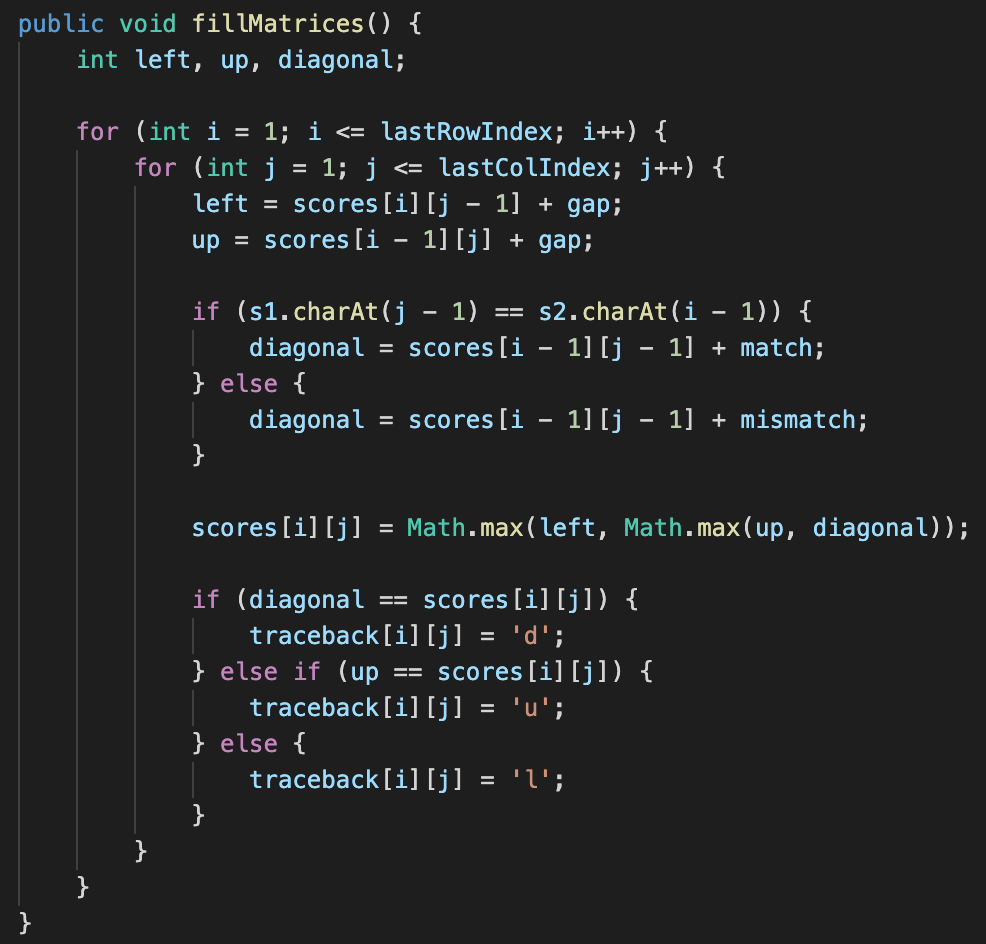
\includegraphics{Figures/9.png}}}
\caption{The fillMatrices() method of our sequential Needleman-Wunsch implementation.}
\label{9}
\end{figure}

The scoring scheme for each implementation is defined at the start of the program. We decided to assign +1 for each match, -1 for each mismatch, and -1 for each gap. These values are stored in variables at the start of the program.

All implementations of the algorithm (both sequential and concurrent) contain the same printOptimal() method that prints the optimal alignment to the screen. Fig.~\ref{10} shows the code for this method. The method recursively traces the completed traceback matrix starting from the bottom rightmost cell of the matrix and inserts gaps into the sequences accordingly. It then recursively prints the results to the screen. Fig.~\ref{11} shows an example output. The sequences are displayed vertically. For example, the first sequence in the example output is ––GT–TA.

\begin{figure}[htbp]
\centerline{\scalebox{.5}{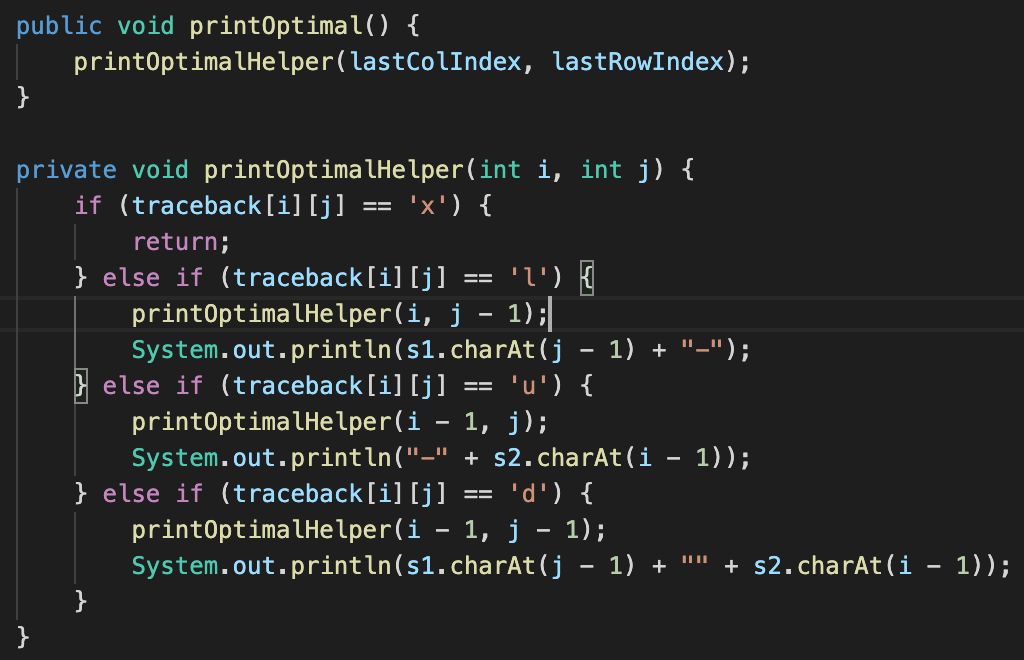
\includegraphics{Figures/10.png}}}
\caption{The printOptimal() method used in all Needleman-Wunsch implementations.}
\label{10}
\end{figure}

\begin{figure}[htbp]
\centerline{\scalebox{.8}{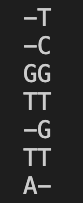
\includegraphics{Figures/11.png}}}
\caption{Example optimal alignment output.}
\label{11}
\end{figure}

In our parallelized versions of the algorithm, we fill in the matrices anti-diagonally. This was achieved by using a nested loop. The outer loop traverses each anti-diagonal starting from the top left and ending at the bottom right. The inner loop, meanwhile, traverses each cell in an anti-diagonal starting from the topmost cell and ending in the leftmost cell.

We ran a sequential version of the algorithm where the matrices are filled in anti-diagonally and found that there was no significant difference in runtime when compared to filling in the matrices in order from left to right starting from the top. Thus, the order of traversal should not affect the runtime.

For all implementations, we tested the results using a pair of short DNA sequences and a pair of long DNA sequences. The short sequences each consists of 15 characters, and the long sequences each consists of 8,191 characters. These sequences are stored in a text file and are read into strings at the beginning of each implementation.

In each parallel version of the algorithm, we run a loop to check the resulting score matrix against the one produced in the sequential version to make sure that the correct output is produced.

\subsubsection{Experiment 1}
In our first attempt to parallelize the Needleman-Wunsch algorithm, we initially tried using locks. Our initial thought was to lock each anti-diagonal. We attempted to use locks to prevent the next anti-diagonal from being processed until the current one is completely filled in. After some time, we realized that this was the wrong approach because of the nature of locks. Locking access to each anti-diagonal meant that only one thread could enter the anti-diagonal at a time. We want all threads to be able to process the anti-diagonal at the same time. As for when processing each cell, there is no need to lock each cell since we are just calculating and filling in the score for the cell. Doing this does not affect the scores of any of the other cells within the same anti-diagonal. We realized that there is no need for locks at all.

This led us to experimenting with atomic variables instead. Knowing that atomic variables are expensive, we tried to come up with an implementation that only required the use of one atomic variable. In order to do this, however, we had to create new threads for each anti-diagonal, which we thought might be even more costly than using multiple atomic variables. Nevertheless, we proceeded with the experiment.

In the implementation, we use an atomic variable to keep track of the current row in each anti-diagonal that still needs to be calculated. The score for each cell is calculated the same way it is in the sequential implementation. The main steps are as follows. First, we traverse to the next anti-diagonal that needs to be processed. We then create 8 new threads and have the main process wait until all 8 threads terminate before looping and traversing to the next anti-diagonal. Each of the created threads enter another loop that traverses the rows in the anti-diagonal. This is equivalent to traversing each cell of the anti-diagonal since each of those cells is on a different row. Every time a thread loops, it calls getAndIncrement() on the current row atomic variable to get the row of the cell it needs to process. It processes the cell assigned to it by calculating the cell's score and updating the scores and traceback matrices. This inner loop continues until there are no more cells to process for the current anti-diagonal. At this point, all threads terminate and the main process proceeds to loop to the next anti-diagonal. Eight new threads are created for this anti-diagonal and the steps are repeated until the matrices are filled. Fig.~\ref{12} shows the outer loop in the implementation. The inner loop is within the run() method, which gets called when each thread runs.

\begin{figure}[htbp]
\centerline{\scalebox{.47}{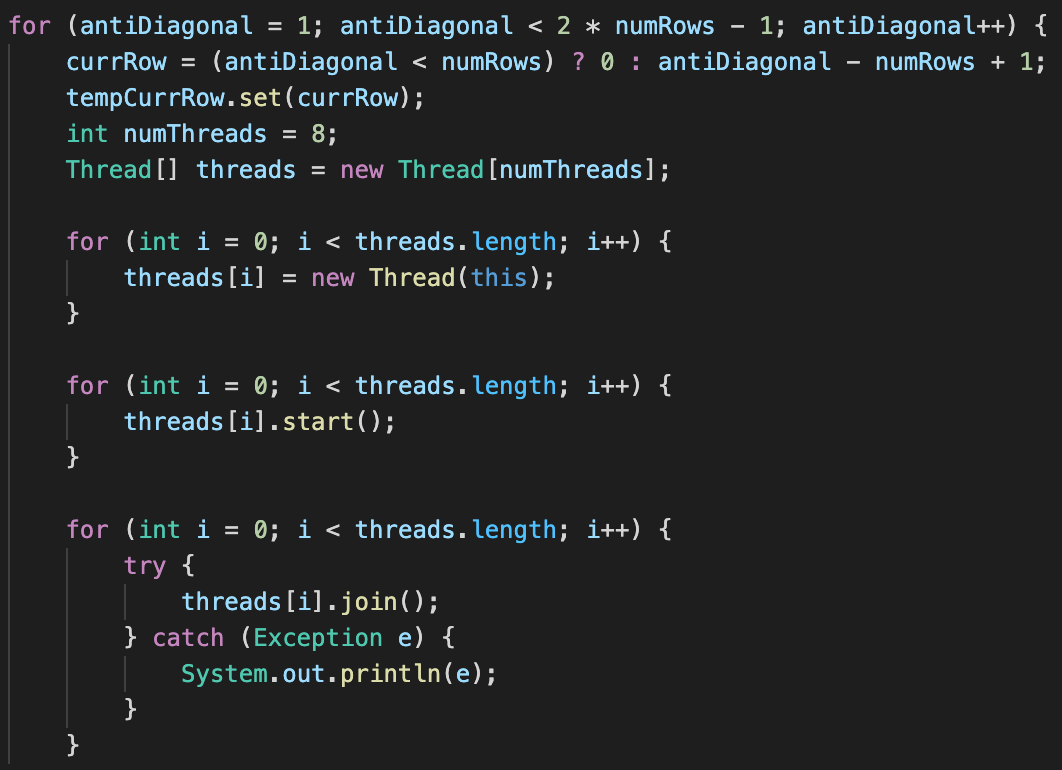
\includegraphics{Figures/12.png}}}
\caption{Portion of Experiment 1 code.}
\label{12}
\end{figure}

Table~\ref{tab:table1} shows the results of Experiment 1 using both the short and long DNA sequence pairs. As can be seen, the runtimes for the sequential implementation is significantly better than the parallel implementation in all cases. To isolate the issue, we removed the multi-threading part of the code and ran the program again to test the impact of only the atomic variable. The execution time for the sequential version here was 1973885 ns, while the execution time for the version with the atomic variable was 2329790 ns. There was a decrease in performance here, but not as nearly significant as before. This shows that the constant creating and terminating of new threads in the Experiment 1 implementation contributed significantly to its slow runtime.

\begin{table}[]
\caption{Experiment 1 results.}
\label{tab:table1}
\begin{tabular}{|l|l|l|l|l|}
\hline
               & \textbf{}      & \textbf{Sequential} & \textbf{Parallel} & \textit{\textbf{Speed Up}} \\ \hline
\textbf{Short} & \textit{Run 1} & 462574 ns           & 18238115 ns       & 0.025363036                \\ \hline
               & \textit{Run 2} & 487001 ns           & 18840366 ns       & 0.025848808                \\ \hline
               & \textit{Run 3} & 469271 ns           & 20105765 ns       & 0.023340123                \\ \hline
\textbf{Long}  & \textit{Run 1} & 629235385 ns        & 7483184535 ns     & 0.08408658                 \\ \hline
               & \textit{Run 2} & 585775817 ns        & 7559493370 ns     & 0.077488765                \\ \hline
               & \textit{Run 3} & 619996746 ns        & 7559426547 ns     & 0.08201637                 \\ \hline
\end{tabular}
\end{table}

\subsubsection{Experiment 2}
In our second attempt to parallelize the algorithm, we moved the thread creation portion of the code to the outside of the loop so that it occurs only once. To prevent the outer loop from going to the next anti-diagonal before it's ready to be processed, we had to use two atomic booleans and another atomic integer in addition to the atomic integer used in the previous experiment that was keeping track of the current row. That's a total of 4 atomic variables being used. Despite atomic variables being costly, we thought that the parallelization would offset this cost.

The first atomic boolean, \emph{waitToLoopAgain}, is used to prevent the threads from moving on to the next anti-diagonal before the current one is processed. It is initially set to true. As seen in Fig.~\ref{13}, we placed a while loop that spins on \emph{waitToLoopAgain} to prevent the threads from moving on until the last cell in the current anti-diagonal is processed. The point at which all the cells in the anti-diagonal is processed is the point when the last thread exits the inner loop. To keep track of this, we used the atomic integer \emph{threadCount} to keep count of the number of threads that has exited the inner loop. Once the last thread has exited the inner loop, we have that thread update some variables to prepare for the processing of the next anti-diagonal. The last thread also sets \emph{waitToLoopAgain} to false to free the other threads from the spin wait. If we loop again directly from this point, a potential problem is that the last thread might become stuck at this point when we reset \emph{waitToLoopAgain} to true again some point before calculating the next anti-diagonal. For instance, if we were to reset \emph{waitToLoopAgain} at the beginning right before the inner loop, one of the other threads might reach the reset point before that last thread is able to get past the spin wait, causing it to be stuck in the last loop iteration. To solve this problem, we introduced another atomic boolean \emph{waitToExecuteLoop}, which guarantees that last thread will always move on to the next iteration. This allows the last thread to be the thread that reset \emph{waitToLoopAgain}. The main downside of this method is that we have to call incrementAndGet() for each thread again in order to keep count of the number of threads that has exited the spin wait on \emph{waitToLoopAgain}. This adds to the overall cost.

\begin{figure}[htbp]
\centerline{\scalebox{.5}{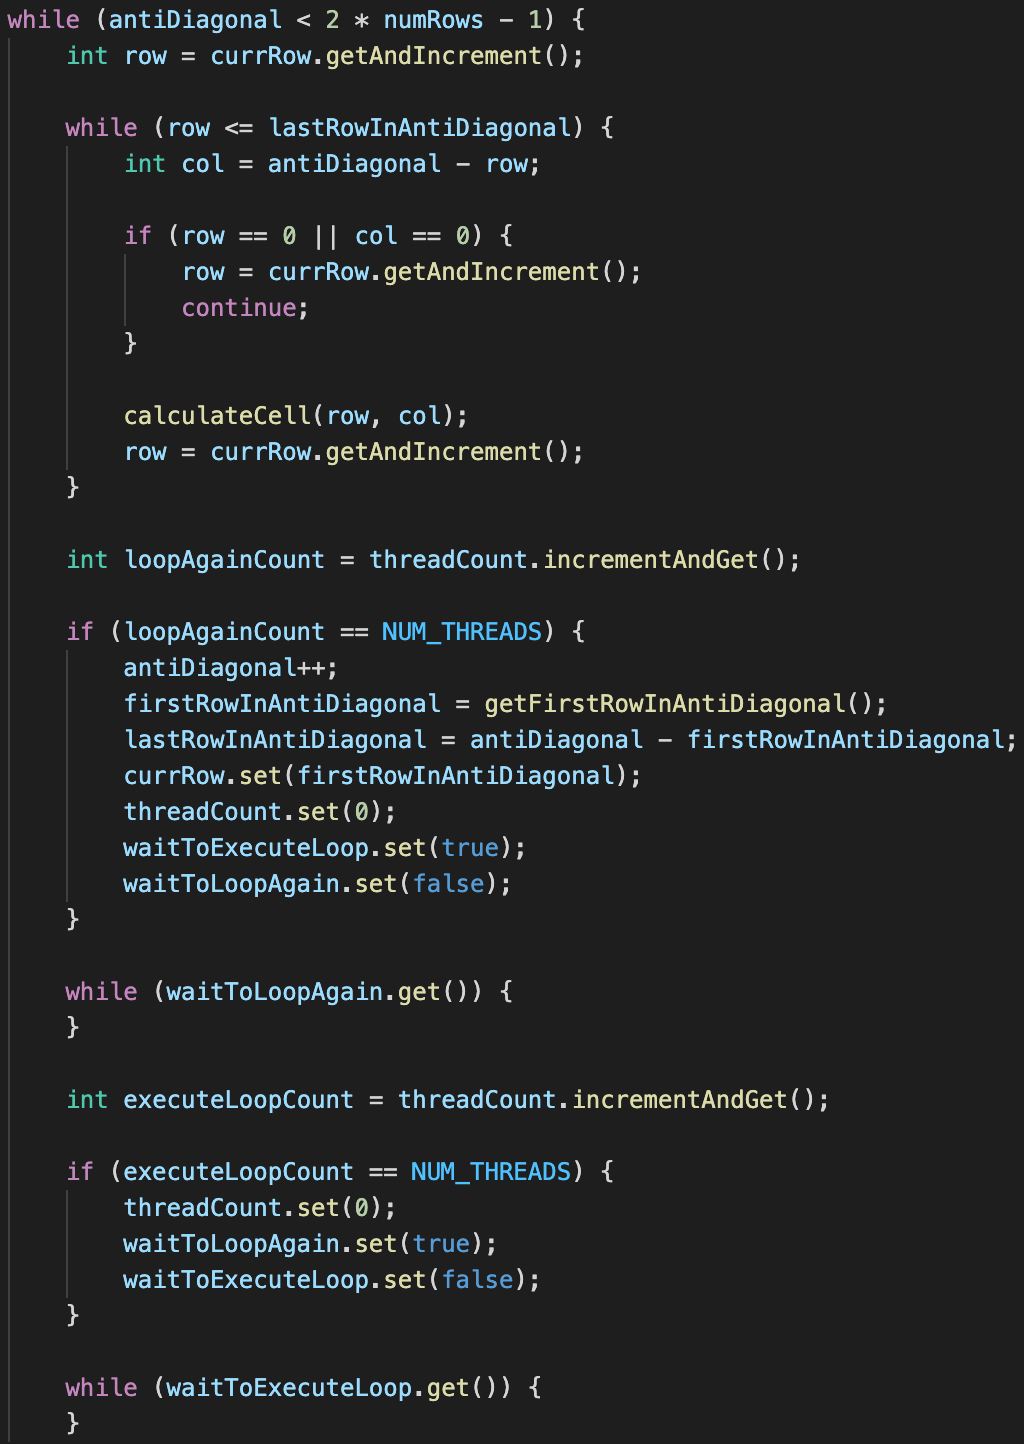
\includegraphics{Figures/13.png}}}
\caption{Portion of Experiment 2 code.}
\label{13}
\end{figure}

Table~\ref{tab:table2} shows the results of Experiment 2. Again, in all cases, the sequential runtimes are much better than the parallel runtimes. The results here are definitely an improvement over those from Experiment 1. The use multiple atomic variables over constantly creating new threads did have a positive effect on runtimes. However, parallelization did not offset the cost of using all of those atomic variables. We performed a small experiment by testing the effects of atomic variable initialization on runtime and found that just initialization alone slowed down runtime. The more atomic variables we initialized, the more the runtime suffered. So this along with all the getAndIncrement()'s we used within the loops definitely contributed to the dismal results.

\begin{table}[]
\caption{Experiment 2 results.}
\label{tab:table2}
\begin{tabular}{|l|l|l|l|l|}
\hline
               & \textbf{}      & \textbf{Sequential} & \textbf{Parallel} & \textit{\textbf{Speed Up}} \\ \hline
\textbf{Short} & \textit{Run 1} & 572938 ns           & 4841669 ns        & 0.118334815                \\ \hline
               & \textit{Run 2} & 500059 ns           & 3022491 ns        & 0.16544598                 \\ \hline
               & \textit{Run 3} & 484493 ns           & 2832178 ns        & 0.17106728                 \\ \hline
\textbf{Long}  & \textit{Run 1} & 667113765 ns        & 2022222281 ns     & 0.3298914                  \\ \hline
               & \textit{Run 2} & 591880250 ns        & 1708562826 ns     & 0.34641996                 \\ \hline
               & \textit{Run 3} & 600636087 ns        & 1812491761 ns     & 0.33138692                 \\ \hline
\end{tabular}
\end{table}

\subsubsection{Experiment 3}
In our third attempt to parallelize the algorithm, we attempt to make use of Java's ExecutorService. Java's ExecutorService creates and manages a pool of threads so that we don't have to manage them ourselves \cite{baeldung_2021}. It then allows us to set tasks to it that are to be run. We thought that perhaps ExecutorService would manage the parallelization better than we did in Experiment 2. To use ExecutorService, it first needs to be instantiated with the number of threads passed in as an argument. We can then use the submit() method to pass in a function that is to be run. Once done, we need to call the shutdown() method to terminate the threads. Otherwise, it will run indefinitely.

Initially, we instantiated the executor outside of the outer loop that traverses the anti-diagonals. We placed the submit() method call inside the inner loop that traverse the cells within each anti-diagonal. We pass to it a lambda function that calculates the cell scores. After a few runs the program, we got the an incorrect output. The matrix produced by the parallel implementation did not match the one produced by the sequential one. This means that the executor isn't always filling in the cells in the order that we expect it to. To remedy this, we moved the instantiation of the executor to the inside of the outer loop. Fig.~\ref{14} shows this. Moving the instantiation fixed the issue. However, now threads are being created every iteration of the outer loop. This is a situation similar to that of Experiment 1.

\begin{figure}[htbp]
\centerline{\scalebox{.47}{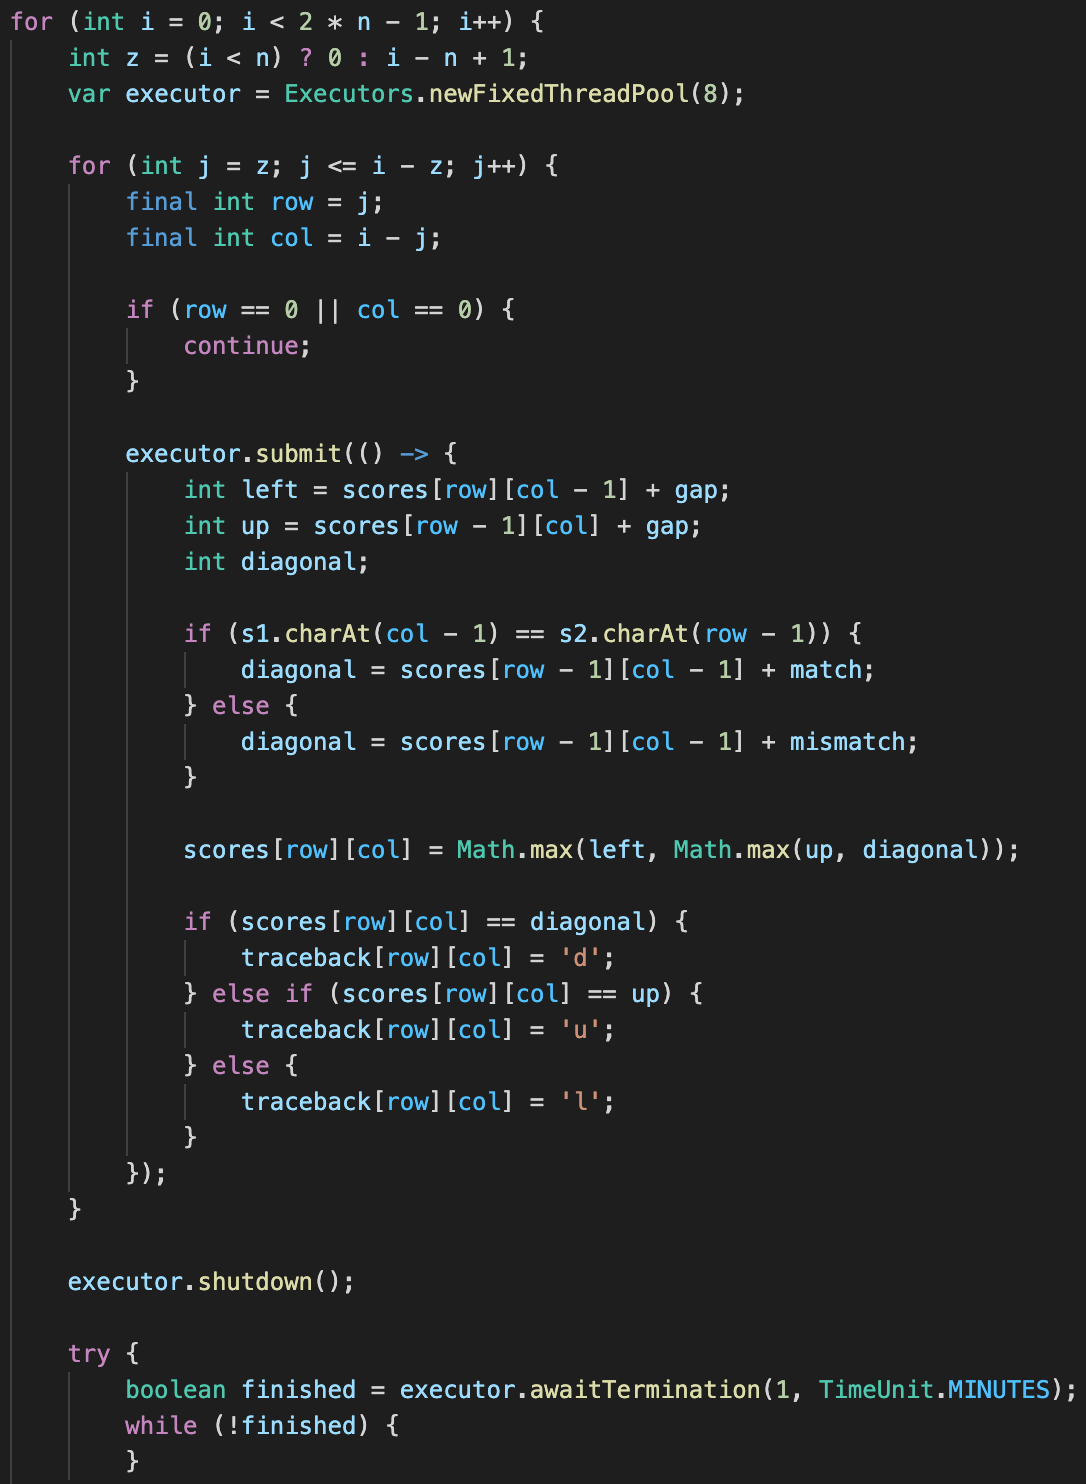
\includegraphics{Figures/14.png}}}
\caption{Portion of Experiment 3 code.}
\label{14}
\end{figure}

Table~\ref{tab:table3} shows the results of Experiment 3. As expected, the results are similar to those of Experiment 1 where the parallel runtimes are significantly higher than the sequential ones due to the constant creation of new threads. Our attempt to use Java's ExecutorService to manage threads did not lead to an improvement over Experiment 2.

\begin{table}[]
\caption{Experiment 3 results.}
\label{tab:table3}
\begin{tabular}{|l|l|l|l|l|}
\hline
               & \textbf{}      & \textbf{Sequential} & \textbf{Parallel} & \textit{\textbf{Speed Up}} \\ \hline
\textbf{Short} & \textit{Run 1} & 472872 ns           & 33430366 ns       & 0.014144984                \\ \hline
               & \textit{Run 2} & 504970 ns           & 29210923 ns       & 0.017287025                \\ \hline
               & \textit{Run 3} & 474302 ns           & 28252854 ns       & 0.016787756                \\ \hline
\textbf{Long}  & \textit{Run 1} & 650375441 ns        & 22830851413 ns    & 0.028486691                \\ \hline
               & \textit{Run 2} & 603525660 ns        & 21543061968 ns    & 0.02801485                 \\ \hline
               & \textit{Run 3} & 596988249 ns        & 21576963582 ns    & 0.02766785                 \\ \hline
\end{tabular}
\end{table}

\subsubsection{Experiment 4}
In our forth attempt to parallelize the algorithm, we try to make use of Java's IntStream parallel() method. Java streams allows us to work more easily with collections of objects by providing functions such as min(), max(), filter(), sum(), and more \cite{baeldung_2019}. An IntStream allows us to work with integers. Using an IntStream, we can run a parallel for-each loop using the range(), forEach(), and parallel() methods. To do this, we specify the range to iterate through in range() and the code to loop through in forEach(). We also call parallel() to request that the loop runs concurrently.

Fig.~\ref{15} shows our implementation of the algorithm using IntStream parallel(). Here, the outer loop traversing through each anti-diagonal operates as normal. The inner loop is implemented using IntStream parallel(), allowing it to be run concurrently. So the calculations for the cells within each anti-diagonal is done concurrently. In doing this, we were hoping that the stream would do a better job at parallelizing the calculations than we did in Experiment 2.

\begin{figure}[htbp]
\centerline{\scalebox{.48}{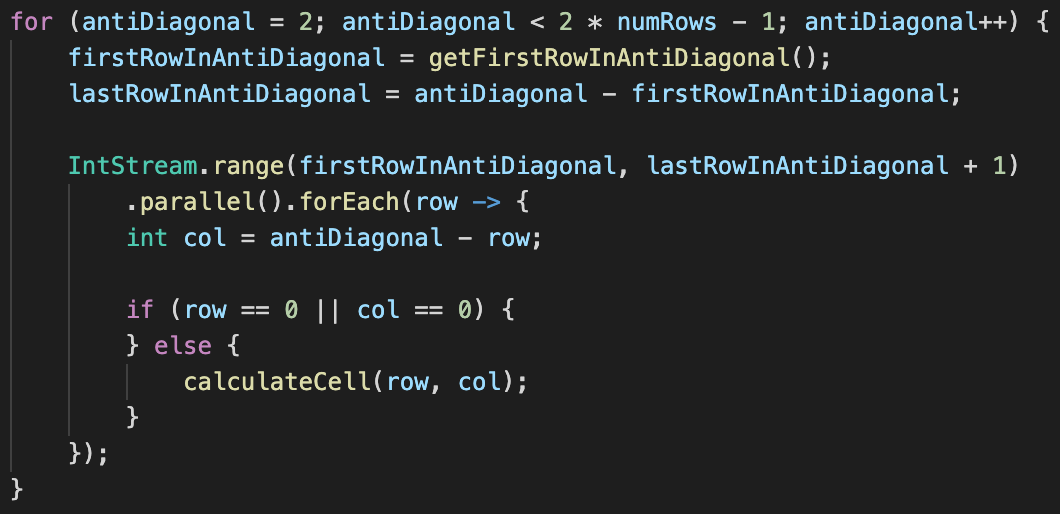
\includegraphics{Figures/15.png}}}
\caption{Portion of Experiment 4 code.}
\label{15}
\end{figure}

Table~\ref{tab:table4} shows the results of Experiment 4. The results are an improvement over those of Experiment 2 for both the short and long DNA sequence pairs. So the stream did indeed do a better job at parallelizing the calculations. However, the sequential runtimes are still at least 2 times faster than the parallel runtimes. The parallel implementation still has not yet won over the sequential one.

\begin{table}[]
\caption{Experiment 4 results.}
\label{tab:table4}
\begin{tabular}{|l|l|l|l|l|}
\hline
               & \textbf{}      & \textbf{Sequential} & \textbf{Parallel} & \textit{\textbf{Speed Up}} \\ \hline
\textbf{Short} & \textit{Run 1} & 471986 ns           & 11916292 ns       & 0.039608464                \\ \hline
               & \textit{Run 2} & 505499 ns           & 12174915 ns       & 0.041519716                \\ \hline
               & \textit{Run 3} & 516278 ns           & 12457773 ns       & 0.041442238                \\ \hline
\textbf{Long}  & \textit{Run 1} & 782632610 ns        & 1298789099 ns     & 0.6025864                  \\ \hline
               & \textit{Run 2} & 594413865 ns        & 1169940500 ns     & 0.5080719                  \\ \hline
               & \textit{Run 3} & 619870475 ns        & 1166825815 ns     & 0.53124505                 \\ \hline
\end{tabular}
\end{table}

These results are the best we have gotten so far. At this point, we considered that maybe we would see improvements if we increased the sizes of the input sequences. Perhaps there is a certain minimum size where we would start seeing the benefits of the parallelized version. We doubled the length of long sequences to be 16,382 characters each and tested the code again. The runtime did not improve. It would stay around the same as before (around 0.5 speed up) and sometimes would even be worse (down to 0.45 speed up).

Next, we attempted to make the code non-blocking by parallelizing both the outer and inner loops to see what would happen. First, we initialized each cell of the score matrix with Integer.MIN\_VALUE. We then implemented the two loops using IntStream parallel() to have them run concurrently. In the calculateCell() method, which determines the score for a cell and gets called in the inner loop, we placed a spin wait on the left, top, and top left diagonal neighbor cells. The spin wait runs until the neighboring cells' values are calculated. That is, it spins until they are not equal to Integer.MIN\_VALUE.

We soon found that the problem with this implementation was that it would almost always lead to a deadlock, especially with the longer sequence. And the reason for this is due to the number of threads spawned by the stream being limited. If all threads land on a cell whose neighbors have not been calculated, they will all spin forever and lead to a deadlock.

\subsubsection{Experiment 5}
In Experiment 5, we attempt to parallelize the initialization of the score and traceback matrices. The first row and column of each matrix are initialized in the constructor. The cells in the first row and column of the score matrix is initialized incrementally based on the gap penalty. If the gap penalty is -5, for example, the first row and column would be as follows: 0, -5, -10, -15,  and so on. The first row of the traceback matrix is initialized with 'u' for up, and the first column is initialized with 'l' for left. Since the initializations of the rows and columns of the matrices are independent, we could use two threads to perform the initializations.

In this experiment, we used two threads to initialize the score and traceback matrices. The first thread initializes the first row of each matrix. The second thread initializes the second row of each matrix. We tested the code on matrices of varying sizes, and the results are shown in Table~\ref{tab:table5}. Initializing 1000 x 1000 sized matrices with the parallel code did not lead to a speed up. The cost of creating the two threads outweighed the benefits of parallelizing. However, once the matrix size reached 10,000 x 10,000, we started seeing a speed up. The parallel initialization here is about 1.2 times  faster than the sequential initialization.

\begin{table}[]
\caption{Experiment 5 results.}
\label{tab:table5}
\begin{tabular}{|l|l|l|l|l|}
\hline
               & \textbf{}      & \textbf{Sequential} & \textbf{Parallel} & \textit{\textbf{Speed Up}} \\ \hline
\textbf{1000 x 1000}   & \textit{Run 1} & 2539679 ns   & 8673331 ns   & 0.29281473 \\ \hline
              & \textit{Run 2} & 2628954 ns   & 8628483 ns   & 0.3046832  \\ \hline
\textbf{5000 x 5000}   & \textit{Run 1} & 64573559 ns  & 66175707 ns  & 0.9757895  \\ \hline
              & \textit{Run 2} & 66140762 ns  & 72408537 ns  & 0.91343874 \\ \hline
\textbf{10000 x 10000} & \textit{Run 1} & 294585528 ns & 236183506 ns & 1.2472739  \\ \hline
              & \textit{Run 2} & 311827281 ns & 243780913 ns & 1.2791293  \\ \hline
\end{tabular}
\end{table}

\section{Others' Implementations}
We looked at some other parallel implementations of the Needleman-Wunsch algorithm that are on GitHub. Most of the implementations were coded in C++ and none were in Java. We thought that maybe the performance would be better in C++. So we ran them to compare the results. The results were similar to ours in that the sequential runtimes were better than the parallel runtimes. One implementation, in particular, is the NW-Parallel project from blakeklasing \cite{blakeklasing}. This implementation was different from ours in that it made use of pools, which was implemented using vectors. We used 2D arrays to represent our matrices. The author initially calculates the first cell, which represents the first anti-diagonal. Once that is done, two items are added to the pool representing the cells below and to the right of the the first cell. Those cells are then calculated. The process continues until all the cells are calculated. The author has a lock-based and lock-free parallel implementation. The lock-based one ran faster than the lock-free one. However, the sequential one ran faster than both parallel ones.

In another implementation, Lee, Kim, and Uy attempted to parallelize and speed up the Needleman-Wunsch algorithm using CUDA. They described their process and results in their paper \cite{lee_kim_uy_2020}. For their serial implementation, they used Java and ran it on a CPU. For their parallel version, they used CUDA C/C++ and ran it on both a CPU and GPU using the anti-diagonal technique. Here, they used vectors to represent the matrices. In the end, they found that their parallel implementation performed three times better than their parallel implementation. So it seems that in order to be able to successfully parallelize the Needleman-Wunsch algorithm, we must make use of a GPU.

\section{Conclusion}
We were able to successfully parallelize the initialization of the matrices in the Needleman-Wunsch algorithm by using different threads to fill in the first rows and the first columns. We were not able to improve performance by parallelizing the calculation of the matrix scores, however.

The calculation of the matrix scores for the Needleman-Wunsch and Smith-Waterman algorithms can only be parallelized within each anti-diagonal. Threads have to be blocked from moving on to the next anti-diagonal until the current anti-diagonal is filled in. In our experiments, we found that the overhead of parallelizing this way wins over the benefits of parallelization. Additionally, increasing the size of the input sequences means increasing the number of anti-diagonals that need to be processed. And the more anti-diagonals there are, the more overhead that is involved. So, it seems that the current heuristic approaches being used right now are the best solutions to the sequence alignment problem even though they do not always return the exact most optimal solutions.

\bibliographystyle{IEEEtran}
\bibliography{IEEEabrv,References}

\end{document}